
The desired point     is given by
   \begin{align}
       \vec{P}&=\myvec{\frac{k\vec{B}+\vec{A}}{k+1}}\\
       &=\frac{\frac{3}{4}\myvec{2\\7}+\myvec{1\\3}}{\frac{3}{4}+1}\\
       &=\frac{1}{7}\myvec{10\\33}
   \end{align}

See Fig. \ref{vec/2006/1/Fig 1.1}.
\begin{figure}[h]
\centering
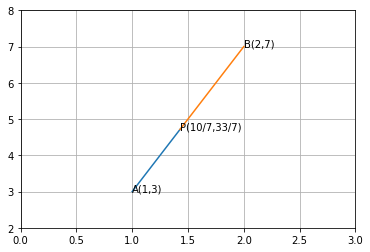
\includegraphics[width=\columnwidth]{vectors/solutions/2006/1/line division.png}
\caption{Two lines representing given equations meet at point $\myvec{2 & -1}$ }.
\label{vec/2006/1/Fig 1.1}
\end{figure}
